\clearpage
\section*{Problem 3}
\markboth{Problem 3}{Problem 3}
\addcontentsline{toc}{section}{Problem 3}

\textbf{Problem Statement:} Consider the linear system $\mathbf{Ax} = \mathbf{b}$, where

$$\mathbf{A} = \begin{bmatrix}
6.25 & -1 & 0.5 \\
-1 & 5 & 2.12 \\
0.5 & 2.12 & 3.6
\end{bmatrix}, \quad \mathbf{b} = \begin{bmatrix}
7.5 \\
-8.68 \\
-0.24
\end{bmatrix}.$$

Write a computer program for LU-factorization with a unit lower triangular $\mathbf{L}$ (meaning that the diagonal entries should be equal to one). Then write a program for the Cholesky factorization.

\textbf{WARNING:} avoid using shortcuts. The programming should be done ``from scratch".

\noindent\rule{\textwidth}{0.4pt}

\vspace{1em}

\textbf{Solution:}

\subsection*{Implementation Approach}

I implemented both LU (Doolittle) and Cholesky factorizations from scratch in Julia, using simple nested loops without any built-in matrix factorization functions. The implementations follow the standard algorithms.

\subsection*{Method 1: LU Factorization}

The LU factorization decomposes $\mathbf{A} = \mathbf{LU}$, where $\mathbf{L}$ is unit lower triangular and $\mathbf{U}$ is upper triangular. Figure~\ref{fig:p03-lu-output} shows the complete output including the factorization, verification, and solution.

\begin{figure}[H]
    \centering
    
\includegraphics[width=0.75\textwidth]{figures/p03-lu-factorization-output.png}
    \caption{LU Factorization output showing the factored matrices $\mathbf{L}$ and $\mathbf{U}$, verification that $\mathbf{A} = \mathbf{LU}$, the computed solution $\mathbf{x}$, and comparison with Julia's built-in solver. The factorization is verified to machine precision ($\sim 10^{-16}$), and the solution matches the built-in solver exactly.}
    \label{fig:p03-lu-output}
\end{figure}

\noindent The factorization yields:
$$\mathbf{L} = \begin{bmatrix}
1.0 & 0.0 & 0.0 \\
-0.16 & 1.0 & 0.0 \\
0.08 & 0.454545 & 1.0
\end{bmatrix}, \quad
\mathbf{U} = \begin{bmatrix}
6.25 & -1.0 & 0.5 \\
0.0 & 4.84 & 2.2 \\
0.0 & 0.0 & 2.56
\end{bmatrix}$$

\noindent Verification: $\max|\mathbf{A} - \mathbf{LU}| = 4.441 \times 10^{-16}$

\subsection*{Method 2: Cholesky Factorization}

The Cholesky factorization exploits the symmetry and positive-definiteness of $\mathbf{A}$, decomposing it as $\mathbf{A} = \mathbf{LL}^T$, where $\mathbf{L}$ is lower triangular. Figure~\ref{fig:p03-cholesky-output} shows the complete output.

\begin{figure}[H]
    \centering
    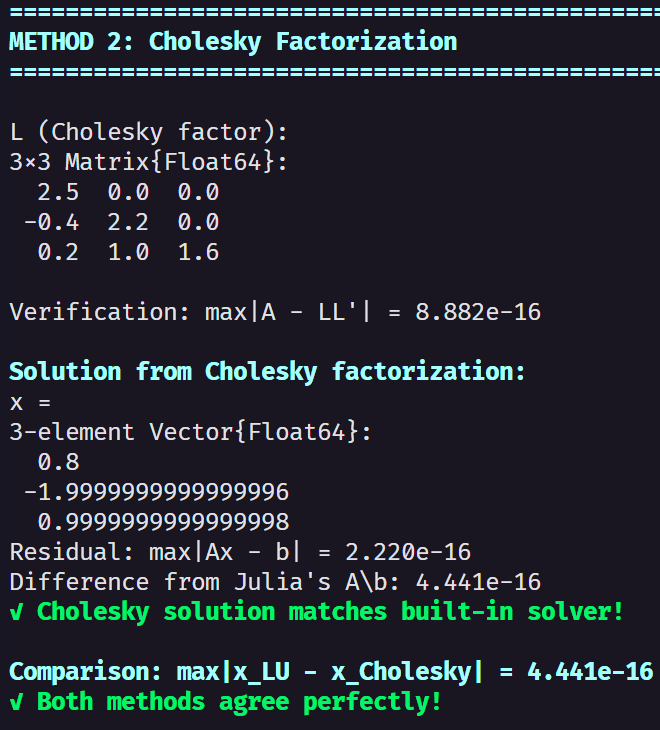
\includegraphics[width=0.75\textwidth]{figures/p03-cholesky-output.png}
    \caption{Cholesky Factorization output showing the Cholesky factor $\mathbf{L}$, verification that $\mathbf{A} = \mathbf{LL}^T$, the computed solution $\mathbf{x}$, and comparison with Julia's built-in solver. The factorization is verified to machine precision, and both LU and Cholesky methods produce identical solutions.}
    \label{fig:p03-cholesky-output}
\end{figure}

\noindent The Cholesky factor is:
$$\mathbf{L}_{\text{Cholesky}} = \begin{bmatrix}
2.5 & 0.0 & 0.0 \\
-0.4 & 2.2 & 0.0 \\
0.2 & 1.0 & 1.6
\end{bmatrix}$$

\noindent Verification: $\max|\mathbf{A} - \mathbf{LL}^T| = 8.882 \times 10^{-16}$

\subsection*{Final Solution}

Both methods yield the same solution (verified to machine precision):

$$\boxed{\mathbf{x} = \begin{bmatrix}
0.8 \\
-2.0 \\
1.0
\end{bmatrix}}$$

\vspace{2em}
\noindent\rule{\textwidth}{0.4pt}
